% Carried over verbatim from monograph/main.tex (Study 1 record, 13 Sep 2026).
\chapter{Verification against the acceptance contract}\label{s1:ch:ch14_verification_against_the_acceptance_cont}

\section{Gate-by-gate status}

\begin{figure}[H]
\centering
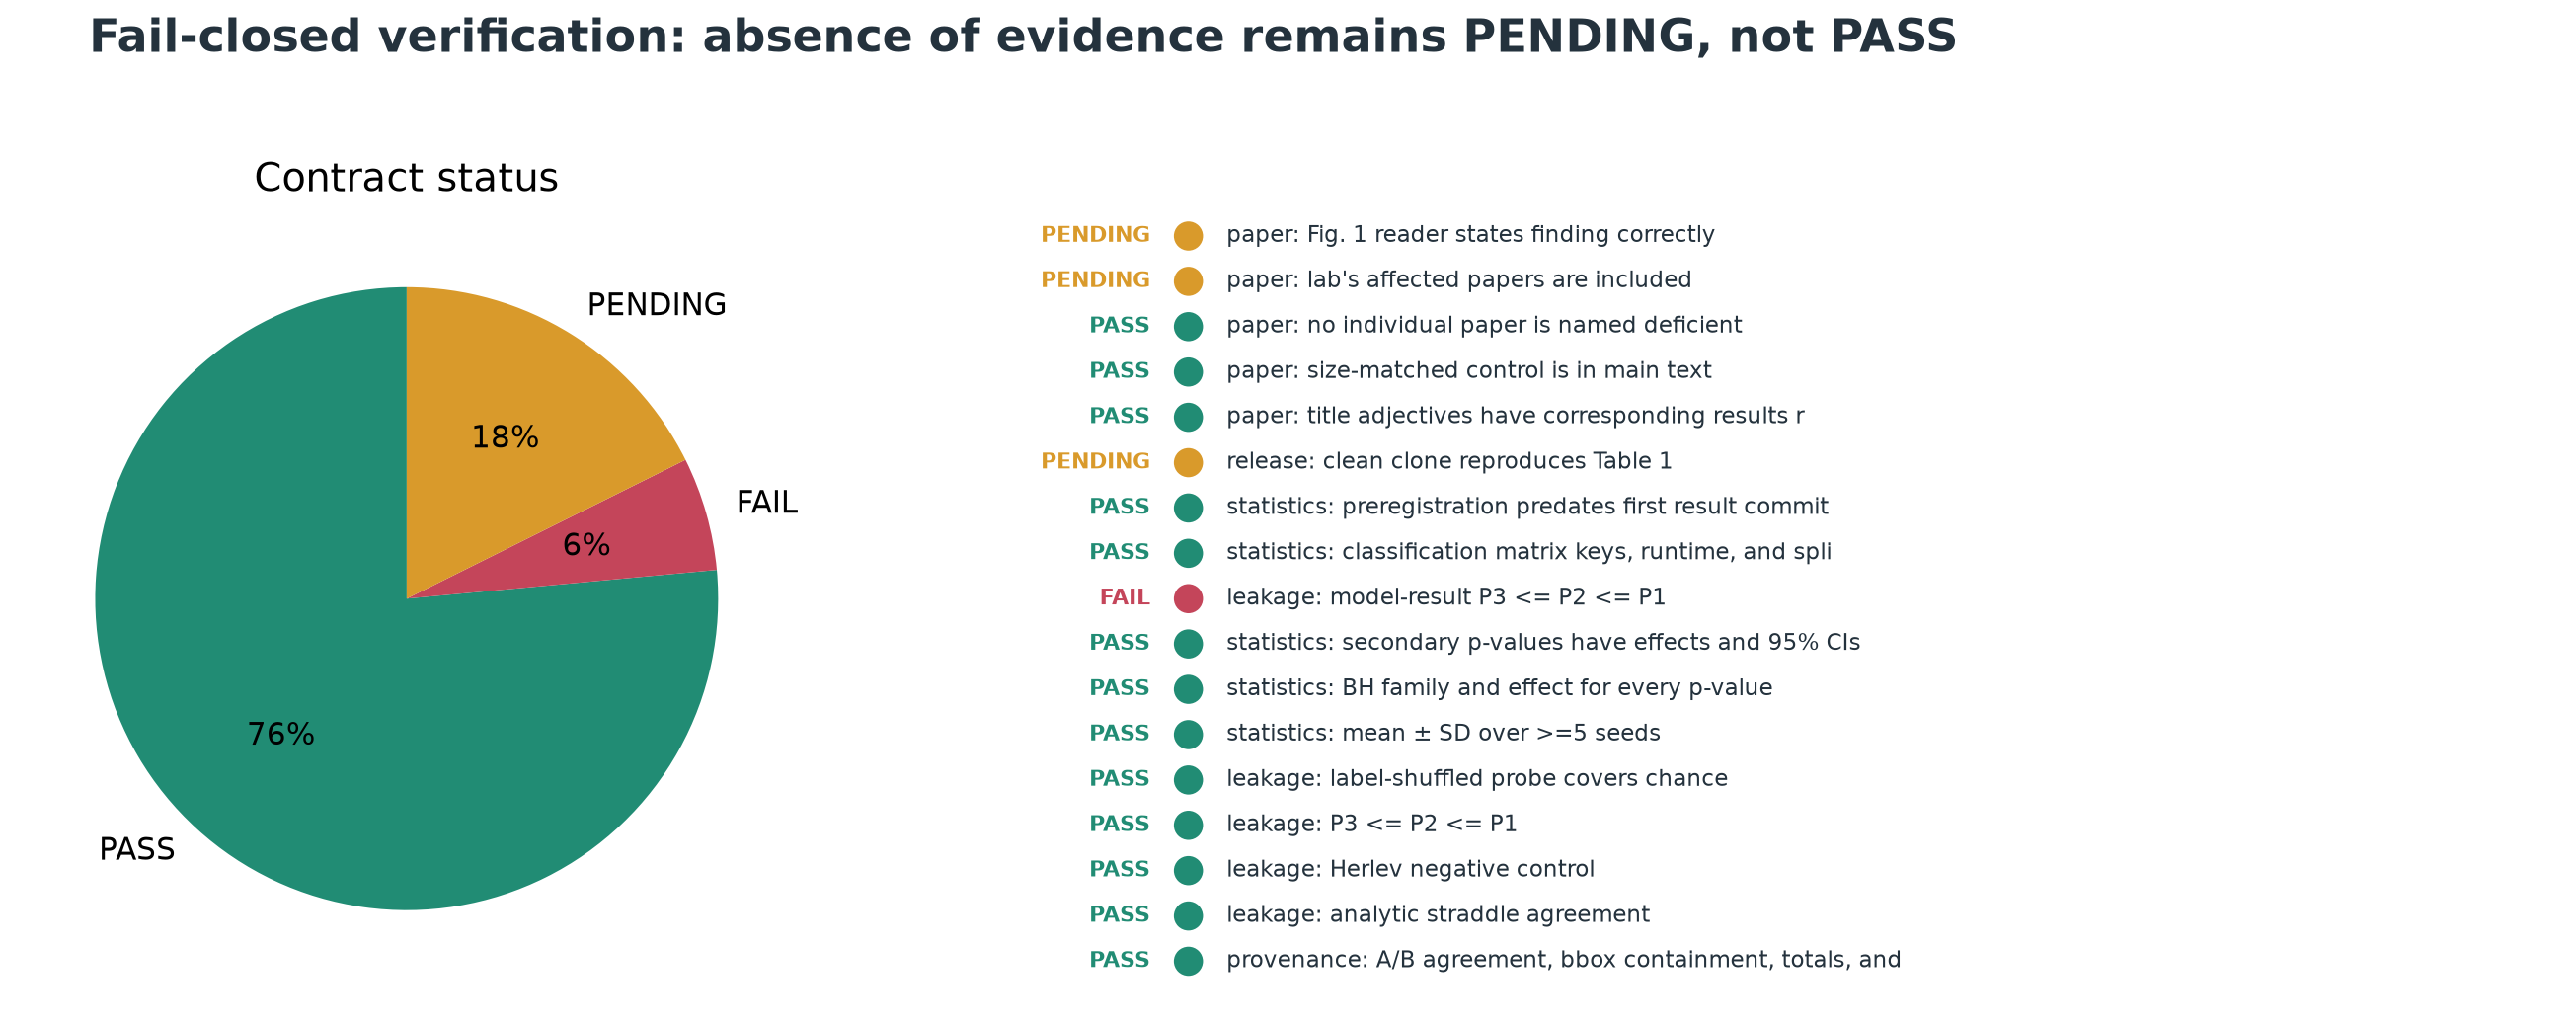
\includegraphics[width=\textwidth]{acceptance_dashboard.png}
\caption{Machine-readable acceptance status: 13 gates pass, one fails, and three remain pending. A pending release gate is not painted green simply because the numerical experiments are complete.}
\label{s1:fig:acceptance}
\end{figure}

\begin{longtable}{p{0.29\textwidth}p{0.14\textwidth}p{0.45\textwidth}}
\caption{Acceptance contract with evidence.}
\label{s1:tab:acceptance}\\
\toprule
Gate & Status & Evidence \\
\midrule
\endfirsthead
\toprule
Gate & Status & Evidence \\
\midrule
\endhead
\bottomrule
\endfoot
SIPaKMeD branch agreement $\geq99\%$ & \pass & 4,049/4,049 mappings agree (100\%). \\
Every bbox lies in parent bounds & \pass & 4,049/4,049 pass geometry checks. \\
Crop and per-class parent totals match & \pass & 4,049 crops; parent vector 126/108/238/271/223. \\
Observed straddle matches analytic prediction & \pass & All audited multi-crop datasets fall inside the recorded simulation envelope. \\
Herlev has no structural effect & \pass & All five seeds return exactly zero in \protocol{P1}; \protocol{P2}/\protocol{P3} also zero. \\
\protocol{P3}$\leq$\protocol{P2}$\leq$\protocol{P1}, structural & \pass & Grouped protocols eliminate measured parent sharing. \\
Shuffled probe confirms chance & \pass & 95\% $t$ interval [$-0.1385$, 0.4687]\% contains 0.2358\%. \\
Every neural summary has $\geq5$ seeds & \pass & 120 classifier, 30 probe, and 175 Cx22 files pass matrix completeness. \\
Plan predates first result commit & \pass & 22 Aug 2026 04:54:10 IST versus 13:22:42 IST. \\
BH applied over stated families & \pass & Stored family labels and $q$ values are reproduced from the exact supplied rows. \\
Effect accompanies every inferential $p$ & \pass & $d_z$, rank-biserial, or Kendall $\tau$ is present. \\
Classifier \protocol{P3}$\leq$\protocol{P2}$\leq$\protocol{P1} & \fail & Only ResNet-50 and ViT-B/16 pass; four of six fail. \\
Cx22 model ordering & \pass & All five semantic and two instance rows pass. \\
Official Cx22 parent disjointness & \pass & Multi-Train and Multi-Test have no shared recovered source parent. \\
Virgin-host clean-clone reproduction & \pending & Script exists, but execution evidence from a never-used host is absent. \\
Lab's own affected papers in audit & \pending & No verified crosswalk in the frozen repository. \\
Figure-1-only independent reader & \pending & No documented colleague response in the frozen repository. \\
\end{longtable}

\section{Why the classification ordering gate fails}

The structural ordering and model-score ordering are different propositions. \protocol{P3} has stricter grouping than \protocol{P2}, but it also creates a different balanced partition. Removing a small duplicate-connected component can alter class composition, parent difficulty, and which observations land in test. A finite test set can therefore score higher under the stricter split even though it contains less structural sharing. The failure warns against using monotonic score ordering as a definition of correctness; leakage absence should be checked directly from IDs and components.

\section{Release-readiness boundary}

The repository contains a one-script verification path, but the strongest release criterion requires a truly clean machine that has never held the repository or data. Running the script on the development host, even in a new directory, would not fully establish that environmental condition. This report therefore leaves the release gate pending. The same standard applies to the human communication gate and lab-paper crosswalk: absence of evidence is not converted into a pass.
